\documentclass{../document}

\addbibresource{refs.bib}

\newcommand{\Caltech}{Theoretical Astrophysics 350-17, California Institute of Technology, Pasadena, CA 91125, USA}
  \newcommand{\CaltechId}{1}
\newcommand{\Oberlin}{Department of Physics and Astronomy, Oberlin College, Oberlin, Ohio 44074, USA}
  \newcommand{\OberlinId}{2}
\newcommand{\Cornell}{Cornell Center for Astrophysics and Planetary Science, Cornell University, Ithaca, New York 14853, USA}
  \newcommand{\CornellId}{3}

\fancyhead[OL]{\it Parameter Control in Binary Black Hole Initial Data}
\fancyhead[ER]{\it Parameter Control in Binary Black Hole Initial Data}

\begin{document}
  \thispagestyle{title}

  \begin{center}
    \Large\bf
    Control of Physical Parameters in \\
    Binary Black Hole Initial Data
  \end{center}
    
  \begin{center}
    Iago Mendes$^{\CaltechId,\OberlinId}$
      \orcidlink{0009-0007-9845-8448}
  \end{center}

  \begin{flushleft}
    Mentors:
      Nils Vu$^\CaltechId$
        \orcidlink{0000-0002-5767-3949},
      Mark Scheel$^\CaltechId$
        \orcidlink{0000-0001-6656-9134},
      Saul Teukolsky$^{\CaltechId,\CornellId}$
        \orcidlink{0000-0001-9765-4526}
  \end{flushleft}
   
  \begin{flushleft}
    \footnotesize
    $^\CaltechId$\Caltech \\
    $^\OberlinId$\Oberlin \\
    $^\CornellId$\Cornell
  \end{flushleft}

  \begin{flushleft}
    This report was submitted as part of the Summer Undergraduate Research Fellowship (SURF) program at Caltech.
  \end{flushleft}

  \begin{center}
    (Dated: \today)
  \end{center}

  \section*{Abstract}

    When solving Einstein's equations for Binary Black Holes (BBH) numerically, we split the four-dimensional spacetime into three-dimensional spatial slices and evolve them over time. The first slice is described by solving an Initial Data problem, which is cast as five elliptic partial differential equations in the extended conformal thin-sandwich (XCTS) decomposition. Prior to solving the XCTS equations, we must choose ``free data'' to impose boundary conditions and specify background quantities. This is the approach taken in {\tt SpECTRE}, a parallel code that aims to simulate BBH for the new generations of gravitational wave detectors. After solving the XCTS system, {\tt SpECTRE} runs a horizon finder that measures the masses and spins of the black holes. Additionally, our work extends {\tt SpECTRE}'s capabilities to calculate total energy, momentum, and center of mass as infinite integrals using the Arnowitt-Deser-Misner (ADM) formalism. Typically, we want to choose these physical quantities before running a BBH simulation, but they can only be measured after numerically solving the XCTS equations. To address this, we implemented an iterative scheme in {\tt SpECTRE} that drives the physical parameters to their desired values by adjusting the free data in a quasi-Newton-Raphson method that efficiently computes the Jacobian with Broyden's method.

  \section{Introduction}
    
    In the early twentieth century, Einstein revolutionized the study of gravity by connecting spacetime geometry with physical dynamics. As John Wheeler says, ``Spacetime tells matter how to move; matter tells spacetime how to curve'' \cite{Wheeler}. Being a highly complex theory, many problems of interest only have analytic solutions in special cases with symmetry. In this context, Numerical Relativity emerged as an essential field to solve these problems numerically, allowing us to explore general cases that can be found in the universe. Specifically, simulations of Binary Black Holes (BBH) became very important as gravitational wave detectors were developed, needing to use numerical results to identify and characterize signals in their data \cite{LIGO}.

    Famously, the Einstein equations relate the curvature of spacetime to the stress-energy of matter, forming a system of ten nonlinear partial differential equations (PDEs). With the 3+1 formalism, we can rearrange these equations so that spacetime is described by spacelike three-dimensional slices of constant time \cite{Alcubierre}. In doing so, we find that four out of the ten equations do not involve time derivatives, implying that they are constraints that must be satisfied at all times. The remaining six equations describe an evolution of the constraint-satisfying fields. Using this formalism, the Spectral Einstein Code ({\tt SpEC}) \cite{SpEC} runs BBH simulations by first finding initial data and then running an evolution on them. Over time, as {\tt SpEC} faced more challenging BBH with high mass ratios and spins, several improvements had to be made to the initial data techniques, which are summarized in \cite{Serguei}.
    
    Despite its success in BBH simulations, {\tt SpEC} shows its limitations in more challenging problems, such as binary neutron star mergers and BBH with extreme configurations. In this context, {\tt SpECTRE} \cite{SpECTRE} was created as a codebase that follows a better parallelism model and aims to be more scalable \cite{Kidder}. Previous work has already shown that {\tt SpECTRE} can be faster and more accurate than {\tt SpEC} when performing similar tasks due to its use of parallelism \cite{Vu}. This will be especially needed for the upcoming gravitational wave detectors with higher sensitivity, such as the Cosmic Explorer, the Einstein Telescope and LISA.
    
    As part of an effort to allow researchers to fully simulate BBH in {\tt SpECTRE}, an initial data procedure similar to the one in {\tt SpEC} needs to be completed. This is greatly benefitted by a scalable elliptic solver that was recently developed \cite{Vu}, which can now be used to solve the initial data equations. Be that as it may, before the start of the SURF program, {\tt SpECTRE} did not have a way to enforce specific masses and spins for the black holes or to avoid drifts in their orbital trajectories. This report describes how we addressed these issues.

  \section{Methods}

    \subsection{Free data}

      To find initial data, {\tt SpECTRE} uses the extended conformal thin-sandwich (XCTS) decomposition (see, e.g., \cite{BaumgarteShapiro} for a review), which transforms the constraint PDEs into a system of five elliptic PDEs. Before solving the XCTS equations, we need to specify the conformal spatial metric $\bar\gamma_{ij}$, the extrinsic curvature trace $K$, and their respective time derivatives $\partial_t \bar\gamma_{ij}$ and $\partial_t K$ \cite{BaumgarteShapiro}. There are many methods for specifying these quantities, but the one that has shown to be the most promising for BBH simulations is the superposed Kerr-Schild (SKS) approach \cite{Lovelace2008}, which enforces quasiequilibrium conditions by setting $\partial_t \bar\gamma_{ij}=0$ and $\partial_t K=0$ and specifies $\bar\gamma_{ij}$ and $K$ by superposing two analytic solutions of Kerr-Schild black holes with masses $M^\text{Kerr}_A$ and $M^\text{Kerr}_B$ and with dimensionless spins $\vec\chi^\text{Kerr}_A$ and $\vec\chi^\text{Kerr}_B$.
      
      We also need to choose the centers of the black holes $\vec c_A$ and $\vec c_B$, which we set so that the Newtonian center of mass,
      \begin{equation} \label{eq:CoM-Newtonian}
        \vec C_\text{Newtonian} = \frac{M^\text{Kerr}_A \vec c_A + M^\text{Kerr}_B \vec c_B}{M^\text{Kerr}_A + M^\text{Kerr}_B},
      \end{equation}
      is zero and their relative distance $\vec c_A - \vec c_B = \vec D$, where $\vec D$ is chosen when setting up the simulation. To give us more control of the placement of the black holes, we add a Newtonian center of mass offset $\vec C_0$.

      Having $\bar\gamma_{ij}$, $K$, $\partial_t \bar\gamma_{ij}$ and $\partial_t K$ specified, we can use the elliptic solver on the XCTS equations, three of which will be solved for the shift $\beta^i$ \cite{BaumgarteShapiro}. Similar to any elliptic PDE problem, we have to set boundary conditions before solving these equations. At the domain outer boundary (with radius $R$), we can add a constant velocity $\vec v_0$ to the boundary conditions of the shift:
      \begin{equation} \label{eq:shift-boundary-condition}
        \beta^i|_R = (\vec \Omega_0 \times \vec r)^i + \dot a_0 r^i + v_0^i,
      \end{equation}
      giving us control over the initial kinematics of the binary system.

      \begin{figure}
        \centering
        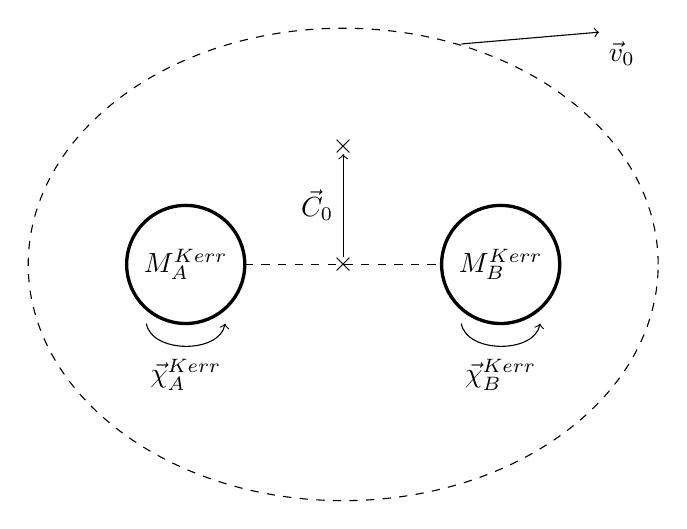
\begin{tikzpicture}[scale=1]
          \draw[very thick] (-2,0) circle (0.75cm);
          \draw[very thick] (+2,0) circle (0.75cm);

          \node at (-2,0) {$M^\text{Kerr}_A$};
          \node at (+2,0) {$M^\text{Kerr}_B$};

          \node at (-2,-1.4) {$\vec\chi^\text{Kerr}_A$};
          \node at (+2,-1.4) {$\vec\chi^\text{Kerr}_B$};

          \draw[->] (-2.5,-0.75) to [out=-80,in=-100] (-1.5,-0.75);
          \draw[->] (1.5,-0.75) to [out=-80,in=-100] (2.5,-0.75);

          \draw[dashed] (-1.25,0) -- (1.25,0);
          \node at (0,0) {$\boldsymbol\times$};
          \node at (0,1.5) {$\boldsymbol\times$};
          \draw[->] (0,0.1) -- (0,1.4) node[pos = 0.5, anchor = east] {$\vec C_0$};

          \draw[dashed] (0,0) ellipse [x radius=4cm, y radius=3cm];
          \draw[->] (1.5,2.8) -- (3.25,2.95) node[pos = 1, anchor = north west] {$\vec v_0$};
        \end{tikzpicture}
        \caption{Schematic representation of the BBH free data.}
        \label{fig:free-data}
      \end{figure}

      Figure \ref{fig:free-data} gives a schematic representation of these free data.

    \subsection{Calculation of asymptotic quantities}

      In Newtonian mechanics, it is typically straightforward to compute the center of mass and the linear momentum of a system. However, in general relativity, these are asymptotic quantities -- defined by infinite surface integrals. Since the computational domains are coarser at their outer boundaries, these integrals tend to be very sensitivity to small errors, leading to less accurate results. To overcome this, we can cast these calculations as volume integrals using Gauss' divergence theorem. Below, we explain the approaches we used to compute these asymptotic quantities in {\tt SpECTRE}.

      We can measure the total energy of a system by computing the ADM mass $M_\text{ADM}$. In terms of conformal quantities, it takes the form of
      \begin{equation} \label{eq:Madm-surf}
        M_\text{ADM}
        = \frac{1}{16\pi} \oint_{S_\infty}  \Big(
          \bar\gamma^{jk} \bar\Gamma^i_{jk}
          - \bar\gamma^{ij} \bar\Gamma_{j}
          - 8 \bar D^i \psi
          \Big) \, d\bar{S}_i
      \end{equation}
      \cite[\eq{3.139}]{BaumgarteShapiro}, where $\bar\Gamma^i_{jk}$ are the Christoffel symbols associated with $\bar\gamma_{ij}$ (see \eq{2.44} in \cite{BaumgarteShapiro} for a definition) and $\bar\Gamma_{j} = \bar\Gamma^{i}_{ij}$. Applying Gauss' theorem to \eq{\eqref{eq:Madm-surf}}, we have
      \begin{align}
        M_\text{ADM}
        &= \frac{1}{16\pi}
            \int_{V_\infty} \bar D_i  \Big(
              \bar\gamma^{jk} \bar\Gamma^i_{jk}
              - \bar\gamma^{ij} \bar\Gamma_{j}
              - 8 \bar D^i \psi
            \Big) \, d\bar{V} \label{eq:Madm-Gauss} \\
        &= \frac{1}{16\pi}
            \int_{V_\infty} \Big(
              \partial_i \bar\gamma^{jk} \bar\Gamma^i_{jk}
              + \bar\gamma^{jk} \partial_i \bar\Gamma^i_{jk}
              + \bar\Gamma_l \bar\gamma^{jk} \bar\Gamma^l_{jk}
              \\ &\qquad\qquad\qquad \notag
              - \partial_i \bar\gamma^{ij} \bar\Gamma_j
              - \bar\gamma^{ij} \partial_i \bar\Gamma_j
              - \bar\Gamma_l \bar\gamma^{lj} \bar\Gamma_j
              - 8 \bar D^2 \psi
            \Big) d\bar{V}, \label{eq:Madm-vol}
      \end{align}
      where we can use the Hamiltonian constraint to replace $8 \bar D^2 \psi$ with
      \begin{equation}
        8 \bar D^2 \psi = \psi \bar R + \frac{2}{3} \psi^5 K^2
                          - \frac{1}{4} \psi^5 \frac{1}{\alpha^2}
                              \Big[ (\bar L \beta)_{ij} - \bar u_{ij} \Big]
                              \Big[ (\bar L \beta)^{ij} - \bar u^{ij} \Big]
                          - 16\pi \psi^5 \rho
      \end{equation}
      \cite[\eq{3.37}]{BaumgarteShapiro}.

      Using the formalism developed in \cite{Baskaran_2003}, we can find the center of mass of a system by evaluating the integral
      \begin{equation} \label{eq:CoM-surf}
        C_\text{CoM}^i = \frac{3}{8 \pi M_\text{ADM}}
                         \oint_{S_\infty} \psi^4 n^i \, dA
      \end{equation}
      \cite[\eq{26}]{Serguei}, where $n^i = x^i / r$ and $r = \sqrt{x^2 + y^2 + z^2}$. Applying Gauss' theorem to \eq{\eqref{eq:CoM-surf}}, we have
      \begin{align}
        C_\text{CoM}^i
        &= \frac{3}{8 \pi M_\text{ADM}}
            \int_{V_\infty} \partial_j \Big( \psi^4 n^i n^j \Big) \, dV \label{eq:CoM-Gauss} \\
        &= \frac{3}{4 \pi M_\text{ADM}}
            \int_{V_\infty} \frac{1}{r^2} \Big(
              2 \psi^3 \partial_j \psi x^i x^j
              + \psi^4 x^i
            \Big) dV. \label{eq:CoM-vol}
      \end{align}

      We can also measure the total linear momentum of a system with the ADM linear momentum $P_\text{ADM}^i$ using the expressions derived in \cite[\eqs{18--22}]{Serguei}. As an infinite surface integral, it is expressed as
      \begin{equation} \label{eq:Padm-surf}
        P_\text{ADM}^i = \frac{1}{8\pi}
                          \oint_{S_\infty} \psi^{10} \Big(
                            K^{ij} - K \gamma^{ij}
                           \Big) \, dS_j.
      \end{equation}
      Applying Gauss' theorem and using the momentum constraint, it becomes
      \begin{align}
        P_\text{ADM}^i
        &= \frac{1}{8\pi}
            \oint_{S_\infty} \partial_j \Big[ \psi^{10} \Big(
              K^{ij} - K \gamma^{ij}
            \Big) \Big] \, dV \label{eq:Padm-Gauss} \\
        &= - \frac{1}{8\pi}
              \int_{V_\infty} \Big[
                \bar\Gamma^i_{jk} P^{jk}
                + \bar\Gamma^j_{jk} P^{jk}
                - 2 \bar\gamma_{jk} P^{jk} \bar\gamma^{il}
                                           \partial_l(\ln\psi)
              \Big] \, dV, \label{eq:Padm-vol}
      \end{align}
      where $P^{ij} = \psi^{10} (K^{ij} - K \gamma^{ij})$ is the integrand of \eq{\eqref{eq:Padm-surf}}. Note that the matter sources are ignored when using the momentum constraint in \cite{BaumgarteShapiro}, but it is straightforward to add the source term to \eq{\eqref{eq:Padm-vol}} is needed in the future.

      An attentive reader might have noticed that we have used Gauss' theorem in two different ways. That is, we used the conformal covariant derivative $\bar D_i$ and the conformal volume element $d\bar{V}$ in \eq{\eqref{eq:Madm-Gauss}}, but the partial derivative $\partial_i$ and the Euclidean volume element $dV$ in \eq{\eqref{eq:CoM-Gauss}} and \eq{\eqref{eq:Padm-Gauss}}. Both approaches are equivalent \cite{DeBenedictis_1998, Teukolsky_2016}, as long as we are consistent.
      
      In practice, {\tt SpECTRE} cannot evaluate volume integrals over all space because the interior of the black holes are excised from the domain. Hence, if we wish to use the infinite volume integrals, we must still perform finite surface integrals enclosing the excisions. For practicality, we choose to do such integrals over the excisions themselves. If we let $S_0$ be the combination of the excision surfaces, the resulting expressions are
      \begin{equation} \label{eq:Madm-mixed}
        \begin{aligned}
        M_\text{ADM}
        &= \frac{1}{16\pi} \oint_{S_0}  \Big(
            \bar\gamma^{jk} \bar\Gamma^i_{jk}
            - \bar\gamma^{ij} \bar\Gamma_{j}
            - 8 \bar D^i \psi
            \Big) \, d\bar{S}_i
            \\ &\quad
            + \frac{1}{16\pi}
            \int_{V_\infty} \Big(
              \partial_i \bar\gamma^{jk} \bar\Gamma^i_{jk}
              + \bar\gamma^{jk} \partial_i \bar\Gamma^i_{jk}
              + \bar\Gamma_l \bar\gamma^{jk} \bar\Gamma^l_{jk}
              \\ &\qquad\qquad\qquad\quad
              - \partial_i \bar\gamma^{ij} \bar\Gamma_j
              - \bar\gamma^{ij} \partial_i \bar\Gamma_j
              - \bar\Gamma_l \bar\gamma^{lj} \bar\Gamma_j
              - 8 \bar D^2 \psi
            \Big) d\bar{V},
        \end{aligned}
      \end{equation}
      \begin{equation} \label{eq:CoM-mixed}
        \begin{aligned}
          C_\text{CoM}^i
          &= \frac{3}{8 \pi M_\text{ADM}}
              \oint_{S_0} \psi^4 n^i \, dA
              \\ &\quad
            +\frac{3}{4 \pi M_\text{ADM}}
              \int_{V_\infty} \frac{1}{r^2} \Big(
                2 \psi^3 \partial_j \psi x^i x^j
                + \psi^4 x^i
              \Big) dV,
        \end{aligned}
      \end{equation}
      \begin{equation} \label{eq:Padm-mixed}
        \begin{aligned}
          P_\text{ADM}^i
          &= \frac{1}{8\pi}
              \oint_{S_0} \psi^{10} \Big(
                K^{ij} - K \gamma^{ij}
              \Big) \, dS_j \\
            &\quad - \frac{1}{8\pi}
              \int_{V_\infty} \Big[
                \bar\Gamma^i_{jk} P^{jk}
                + \bar\Gamma^j_{jk} P^{jk}
                - 2 \bar\gamma_{jk} P^{jk} \bar\gamma^{il}
                                          \partial_l(\ln\psi)
              \Big] \, dV.
        \end{aligned}
      \end{equation}

      Because of {\tt SpECTRE}'s task-based parallelism, we must first evaluate the integrals locally in each domain element. Then, we perform a reduction to combine the results from all elements into a single result for the entire domain.

    \subsection{Control scheme}
      
      Once the XCTS equations are solved, we have all the information that we need about the zero-time slice of spacetime. With this, we can use an apparent horizon finder to get measurements of the black holes in the constructed initial data. Let $M_A$, $M_B$, $\vec\chi_{A}$ and $\vec\chi_{B}$ be the masses and spins of the actual black holes that we have been able to create. In general, these values will differ from the ``target'' quantities $M^*_A$, $M^*_B$, $\vec\chi^*_{A}$ and $\vec\chi^*_{B}$. For example, suppose that we wish to simulate an equal-mass non-spinning case with $M^*_A = M^*_B = 0.5$ and $\vec\chi^*_{A} = \vec\chi^*_{B} = (0,0,0)$. In order to construct the SKS analytical expressions, it is natural to specify $M^\text{Kerr}_{A,B} = M^*_{A,B}$ and $\vec\chi^\text{Kerr}_{A,B} = \vec\chi^*_{A,B}$. With this, we can solve the XCTS equations and find horizons in the resulting initial data. Once we do it in {\tt SpECTRE}, we find that the resulting black hole parameters are actually $M_{A,B} \approx 0.6$ and $\vec\chi_{A,B} \approx (0,0,-0.002)$.

      If we measure the asymptotic quantities described in the previous subsection, we might find that they are also not desirable. Ideally, $\vec C_\text{CoM}$ and $\vec P_\text{ADM}$ should be equal to zero in order to minimize any drifts of the binary orbit, especially for long simulations. However, similar to the example above, we can only know these quantities after the initial data has been constructed.

      Note that $M_{A,B}$, $\vec\chi_{A,B}$, $\vec C_\text{CoM}$ and $\vec P_\text{ADM}$ are the parameters that we wish to control, but we cannot directly set them to the desired values. We handle this issue is by iterating over different choices of the free data ($M^\text{Kerr}_{A,B}$, $\vec\chi^\text{Kerr}_{A,B}$, $\vec C_0$ and $\vec v_0$), trying to find the ones that result in the ideal physical parameters. Figure \ref{fig:control-loop} shows a schematic representation of this ``control loop''.
    
      \begin{figure}
        \centering
        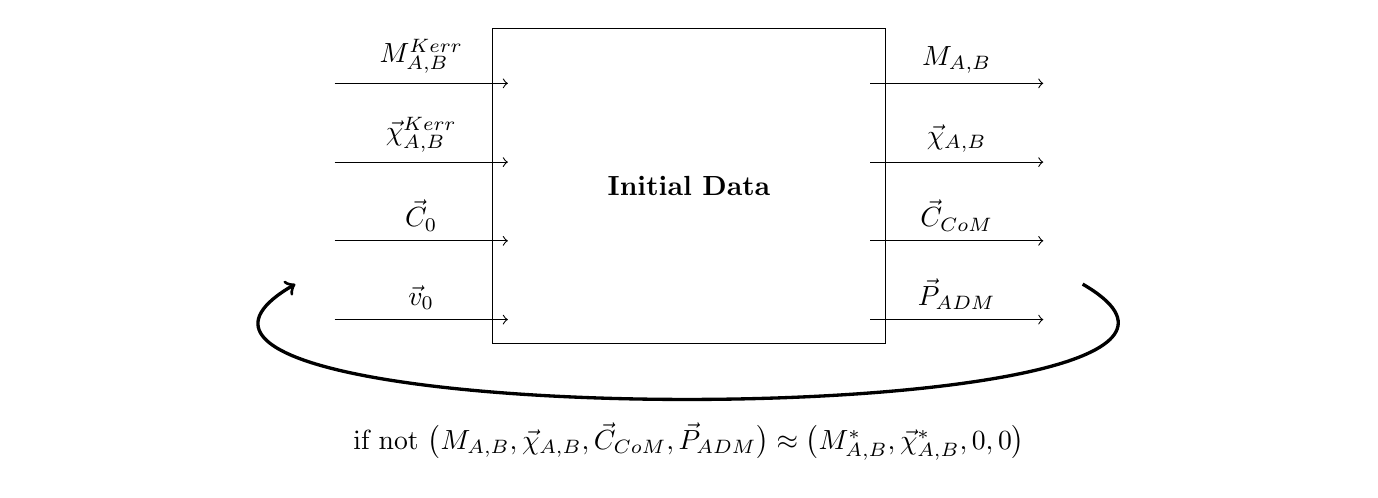
\begin{tikzpicture}
          \node at (0,0) {\bf Initial Data};
    
          \draw (-2.5,-2) rectangle (2.5,2);
    
          \draw[->] (-4.5,1.3) -- (-2.3,1.3) node[anchor = south, pos = 0.5] {$M^\text{Kerr}_{A,B}$};
          \draw[->] (-4.5,0.3) -- (-2.3,0.3) node[anchor = south, pos = 0.5] {$\vec\chi^\text{Kerr}_{A,B}$};
          \draw[->] (-4.5,-0.7) -- (-2.3,-0.7) node[anchor = south, pos = 0.5] {$\vec C_0$};
          \draw[->] (-4.5,-1.7) -- (-2.3,-1.7) node[anchor = south, pos = 0.5] {$\vec v_0$};
    
          \draw[->] (2.3,1.3) -- (4.5,1.3) node[anchor = south, pos = 0.5] {$M_{A,B}$};
          \draw[->] (2.3,0.3) -- (4.5,0.3) node[anchor = south, pos = 0.5] {$\vec\chi_{A,B}$};
          \draw[->] (2.3,-0.7) -- (4.5,-0.7) node[anchor = south, pos = 0.5] {$\vec C_\text{CoM}$};
          \draw[->] (2.3,-1.7) -- (4.5,-1.7) node[anchor = south, pos = 0.5] {$\vec P_\text{ADM}$};
    
          \draw[->, very thick] (5,-1.25) to [out=-30,in=-150] (-5,-1.25);
          \node at (0,-3.25) {if not $\big(M_{A,B}, \vec\chi_{A,B}, \vec C_\text{CoM}, \vec P_\text{ADM}\big) \approx \big(M^*_{A,B}, \vec\chi^*_{A,B}, 0, 0\big)$};
        \end{tikzpicture}
        \caption{Schematic representation of the control loop.}
        \label{fig:control-loop}
      \end{figure}
    
      Let the choices of the free data be represented as
      \begin{equation} \label{eq:u}
        \begin{aligned}
          {\bf u}
          = \Big(
            M^\text{Kerr}_A,
            M^\text{Kerr}_B,
            \chi^{\text{Kerr},x}_A, \chi^{\text{Kerr},y}_A, \chi^{\text{Kerr},z}_A, \qquad\qquad\quad \\
            \chi^{\text{Kerr},x}_B, \chi^{\text{Kerr},y}_B, \chi^{\text{Kerr},z}_B,
            C_0^x, C_0^y, C_0^z,
            v_0^x, v_0^y, v_0^z
          \Big).
        \end{aligned}
      \end{equation}
      Also, let the difference between the current and target physical parameters be represented the ``residual'' function
      \begin{equation}
        \begin{aligned}
          {\bf F}({\bf u})
          = \Big(
            M_A - M^*_A,
            M_B - M^*_B,
            \chi^x_A - \chi^{*,x}_A, \chi^y_A - \chi^{*,y}_A, \chi^z_A - \chi^{*,z}_A, \qquad\qquad\qquad\qquad\quad \\
            \chi^x_B - \chi^{*,x}_B, \chi^y_B - \chi^{*,y}_B, \chi^z_B - \chi^{*,z}_B,
            C_\text{CoM}^x, C_\text{CoM}^y, C_\text{CoM}^z,
            P_\text{ADM}^x, P_\text{ADM}^y, P_\text{ADM}^z
          \Big).
        \end{aligned}
      \end{equation}
      As discussed in the example above, it is natural to use the target values as an initial guess for the free data:
      \begin{equation} \label{eq:u0}
        \begin{aligned}
          {\bf u}_0
          = \Big(
            M^*_A,
            M^*_B,
            \chi^{*,x}_A, \chi^{*,y}_A, \chi^{*,z}_A, \qquad\quad \\
            \chi^{*,x}_B, \chi^{*,y}_B, \chi^{*,z}_B,
            0, 0, 0,
            0, 0, 0
          \Big).
        \end{aligned}
      \end{equation}

      With this, we can update our free data at every control iteration $k \geq 1$ using a Newton-Raphson scheme \cite{NumericalRecipes}:
      \begin{equation}\label{eq:u-iteration}
        {\bf u}_k = {\bf u}_{k-1} - \mathbb{J}^{-1}_{k-1} \cdot {\bf F}_{k-1}.
      \end{equation}
      However, note that each evaluation of ${\bf F}({\bf u})$ is computationally expensive as it requires an entire initial data solve. Therefore, computing the Jacobian in \eq{\eqref{eq:u-iteration}} analytically is unfeasible. That said, we can find it numerically using Broyden's method \cite{NumericalRecipes}:
      \begin{equation}\label{eq:J-iteration}
        \mathbb{J}_k = \mathbb{J}_{k-1} + \frac{{\bf F}_k \otimes \Delta {\bf u}_k}{||\Delta {\bf u}_k||^2},
      \end{equation}
      where $\Delta {\bf u}_k = {\bf u}_k - {\bf u}_{k-1}$.

      Since we're iteratively computing the Jacobian with \eq{\eqref{eq:J-iteration}}, we must choose an adequate initial guess $\mathbb{J}_0$. Assuming that $M_{A,B}|_0 \approx M^\text{Kerr}_{A,B}|_0$ and $\vec\chi_{A,B}|_0 \approx \vec\chi^\text{Kerr}_{A,B}|_0$,
      \begin{equation}
        \frac{\partial (M_{A,B} - M^*_{A,B})}{\partial M^\text{Kerr}_{A,B}}\Bigg|_0
        \approx \frac{\partial (\chi^i_{A,B} - \chi^{*,i}_{A,B})}{\partial \chi^{\text{Kerr},i}_{A,B}}\Bigg|_0
        \approx 1.
      \end{equation}
      Using a Newtonian center of mass approximation,
      \begin{equation}
        \vec C_\text{CoM} \approx \vec C_0,
      \end{equation}
      implying that
      \begin{equation}
        \frac{\partial (C_\text{CoM}^i)}{\partial C_0^i}\Bigg|_0 \approx 1.
      \end{equation}
      We can also use a Newtonian linear momentum approximation with \eq{\eqref{eq:shift-boundary-condition}} as the center-of-mass velocity:
      \begin{equation} \label{eq:P-Newtonian}
        \vec P_\text{ADM} \approx \vec P_\text{Newtonian} = (M_A + M_B) \Big[ (\vec \Omega_0 \times \vec C_\text{CoM}) + \dot a_0 \vec C_\text{CoM} + \vec v_0 \Big],
      \end{equation}
      where $\vec \Omega_0$ is the initial angular velocity and $\dot a_0$ is the initial radial expansion velocity. Typically, these initial orbit parameters are small and $M_A + M_B \approx 1$ in code units. Then,
      \begin{equation}
        \frac{\partial (P_\text{ADM}^i)}{\partial v_0^i}\Bigg|_0 \approx 1.
      \end{equation}
      All the other partial derivatives that go into $\mathbb{J}_0$ are approximately zero under the assumptions imposed above. Therefore, a good initial guess for the Jacobian is
      \begin{equation} \label{eq:J0}
        \mathbb{J}_0 \approx \mathbb{I},
      \end{equation}
      a 14-by-14 identity matrix.

      This control scheme differs from the one used in {\tt SpEC} (see \cite{Serguei}) in a couple of ways. First, instead of the free data in \eq{\eqref{eq:u}}, {\tt SpEC} uses the SKS radii $r_{A}$ and $r_{B}$, the SKS angular velocities $\vec\Omega_{A}^\text{Kerr}$ and $\vec\Omega_{B}^\text{Kerr}$, the center of the larger black hole $\vec c_A$, and the same constant velocity $\vec v_0$ in \eq{\eqref{eq:shift-boundary-condition}}. In theory, our change of controlled variables should lead to equivalent results, but it allows the approximation in \eq{\eqref{eq:J0}} to be made. Second, {\tt SpEC} expands the Newtonian approximations in \eq{\eqref{eq:CoM-Newtonian}} and \eq{\eqref{eq:P-Newtonian}} under perturbations $\delta \vec c_A$ and $\delta \vec v_0$ to derive Newton-Raphson iterations. Here, because of the \eq{\eqref{eq:J0}}, it is straightforward to use Broyden's method for all of our free data, which should converge to the proper Jacobian of ${\bf F}(\bf u)$.
    
  \section{Results}

    \subsection{Convergence of asymptotic quantities}

      We have tested our calculation of asymptotic quantities with analytic solutions of a single black hole, as well as with a numeric solution to the XCTS equations for BBH. The analytic solutions we used describe a Schwarzschild black hole of mass $M$ in isotropic coordinates and in Kerr-Schild coordinates, both with and without a boost speed $v$. The expected values of $M_\text{ADM}$ and $P_\text{ADM}$ for the unboosted solutions are $M_\text{ref} = M$ and $P_\text{ref} = 0$, while the ones for the boosted solutions are $M_\text{ref} = \gamma M$ and $P_\text{ref} = \gamma M v$, where $\gamma = 1 / \sqrt{1 - v^2}$ is the Lorentz factor. We also use a BBH solution for an equal-mass non-spinning case, implying that the expected value of $P_\text{ADM}$ is $P_\text{ref} = 0$. Since we do not know the expected value of $M_\text{ADM}$ for the BBH solution, we use the result at the largest outer radius $R$ as a reference: $M_\text{ref} = M_\text{ADM} |_{\max R}$.

      \begin{figure}
        \centering
        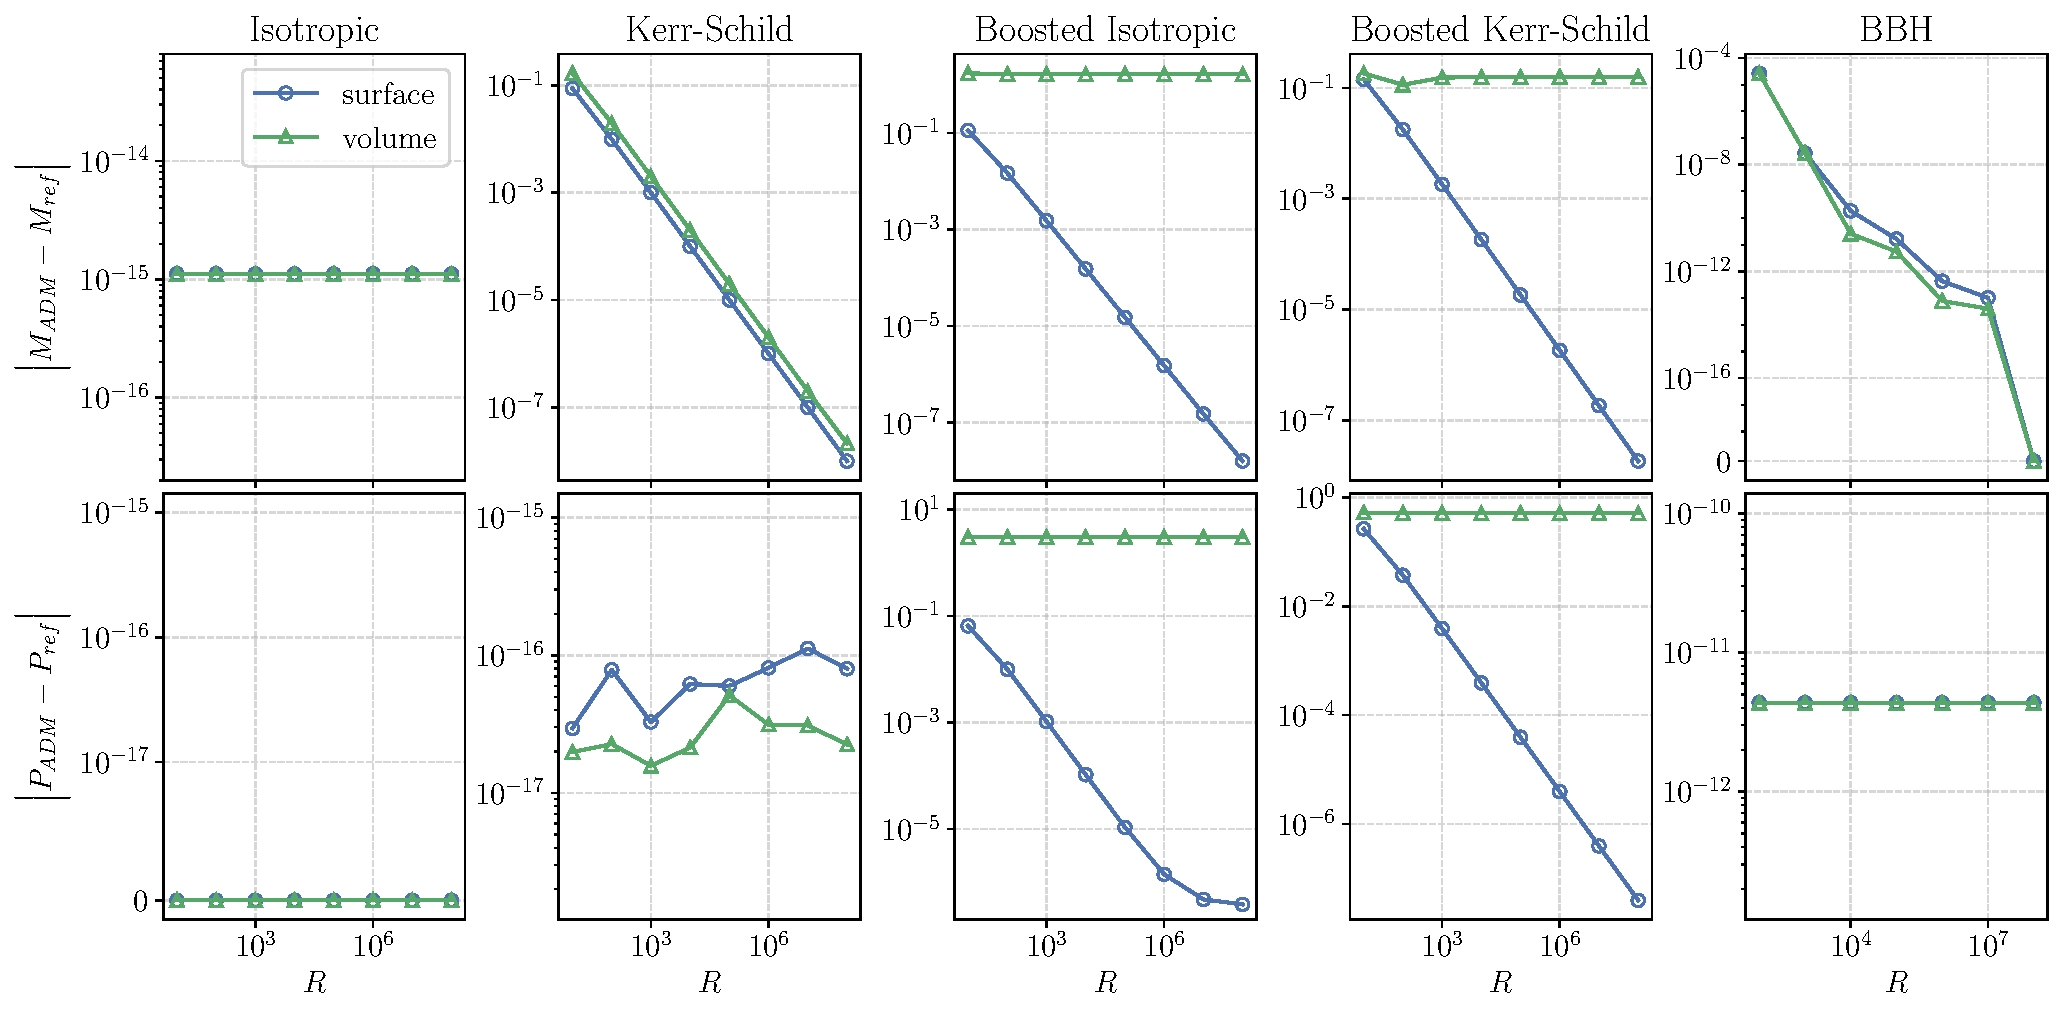
\includegraphics[width=\textwidth]{../../plots/final_report/distance_convergence_Madm_Padm.pdf}
        \caption{Convergence with distance for $M_\text{ADM}$ and $P_\text{ADM}$. ``Surface'' indicates results from evaluating the infinite surface integrals defined in \eq{\eqref{eq:Madm-surf}} and \eq{\eqref{eq:Padm-surf}}. ``Volume'' indicates results from evaluating the finite surface integrals and the infinite volume integrals defined in \eq{\eqref{eq:Madm-mixed}} and \eq{\eqref{eq:Padm-mixed}}.}
        \label{fig:distance_convergence_Madm_Padm}
      \end{figure}

      Figure \ref{fig:distance_convergence_Madm_Padm} compares the difference between the measured $M_\text{ADM}$ and $P_\text{ADM}$ with the reference values $M_\text{ref}$ and $P_\text{ref}$, as described in the previous paragraph. For each subplot, we see how this residual evolves as we increase the outer radius $R$ of the domain, which serves as ``infinity'' in these calculations. Since these quantities are defined asymptotically, we should approach the reference values as $R$ increases. Excluding trivial cases (in which the residuals already start very low), we see that the infinite surface integrals defined in \eq{\eqref{eq:Madm-surf}} and \eq{\eqref{eq:Padm-surf}} converge just as expected. However, this is not the case for the finite surface integrals and infinite volume integrals defined in \eq{\eqref{eq:Madm-mixed}} and \eq{\eqref{eq:Padm-mixed}}. In fact, we see that the results do not converge at all for the boosted cases.  Other than that, this approach behaves as expected.

      \begin{figure}
        \centering
        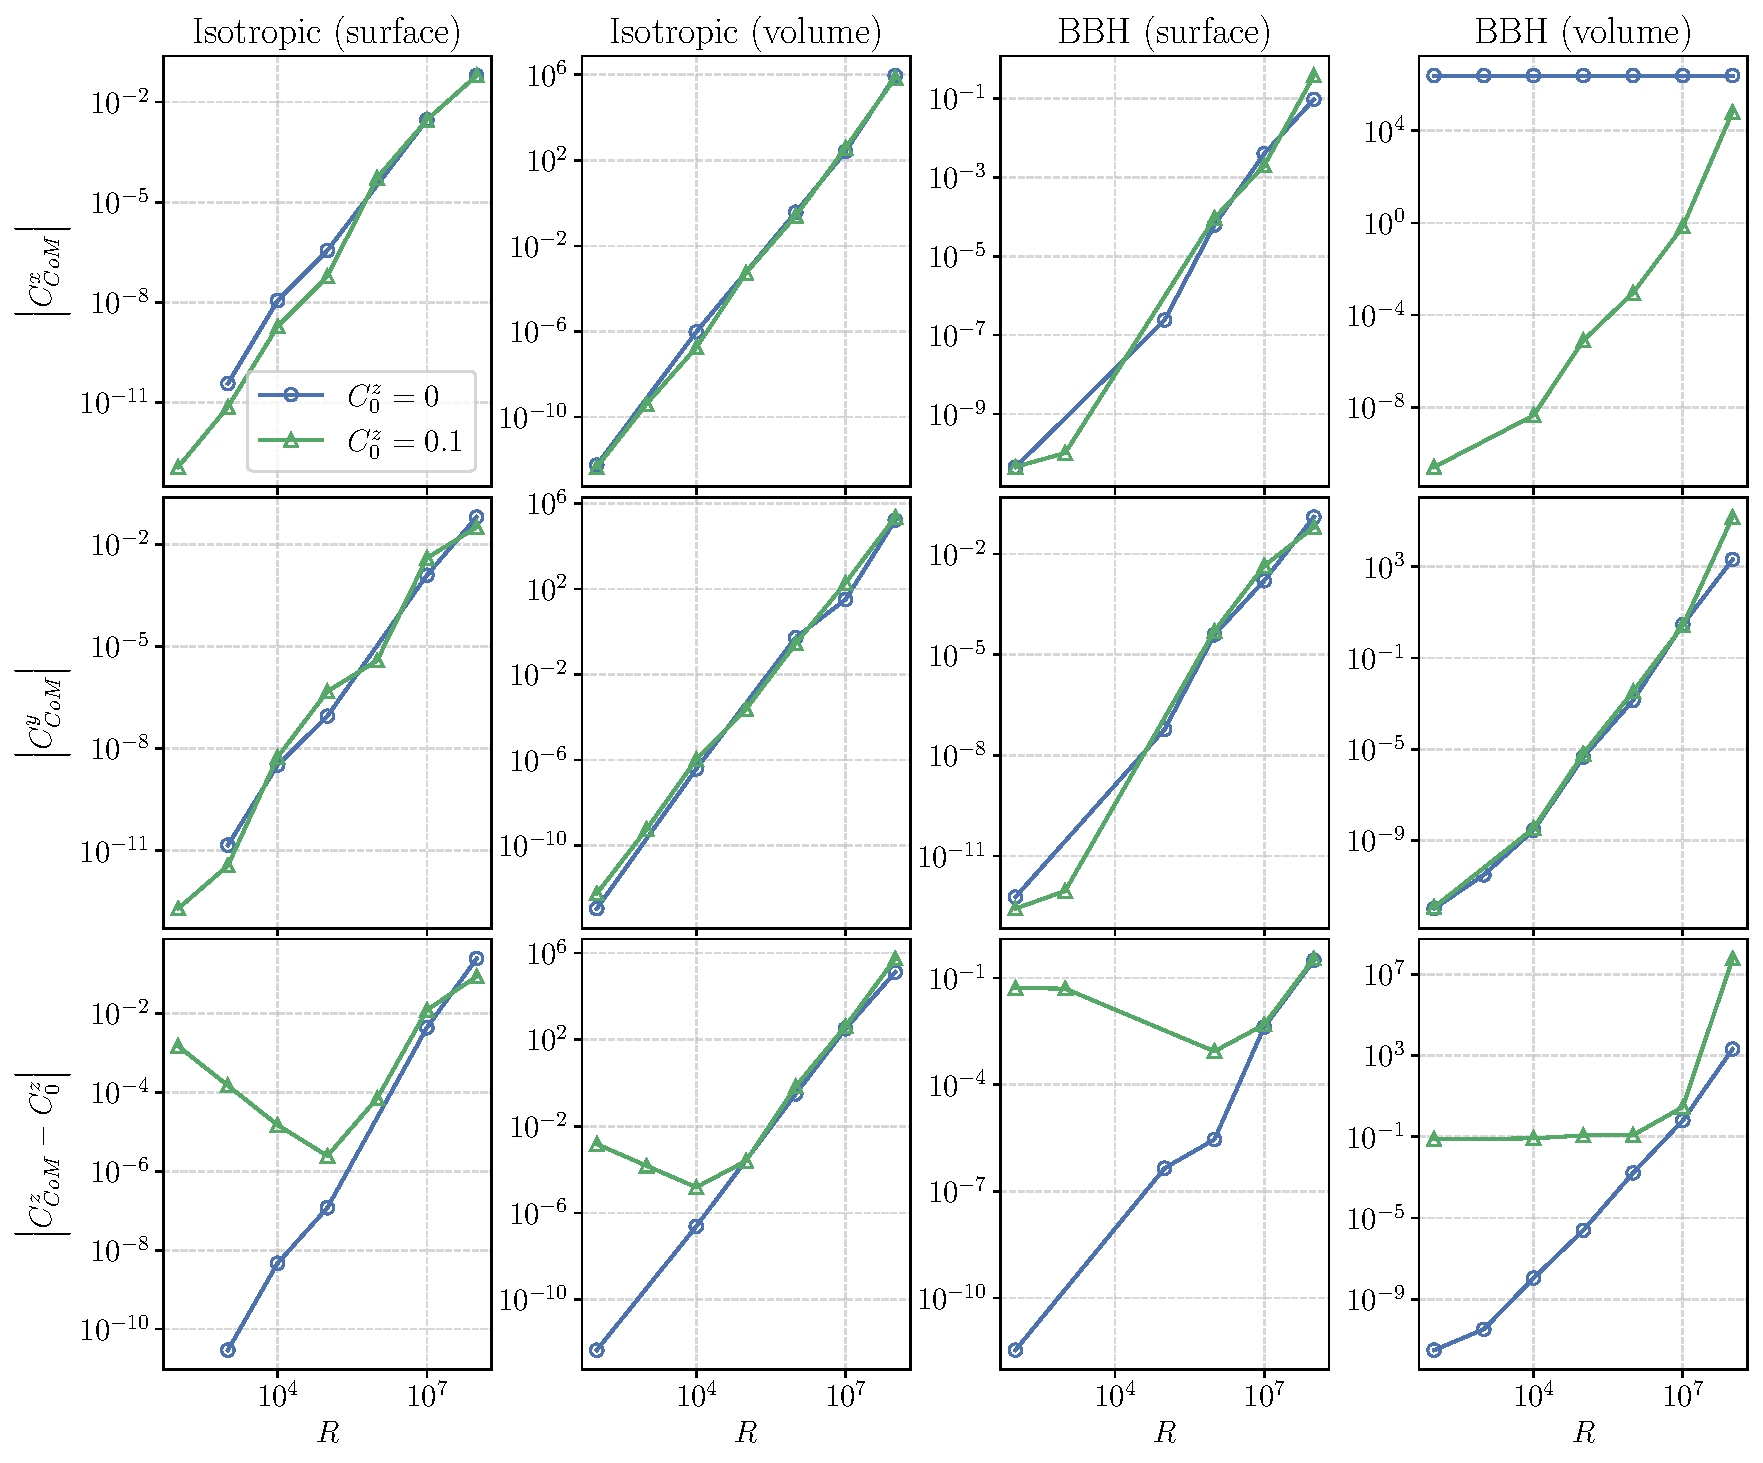
\includegraphics[width=0.85\textwidth]{../../plots/final_report/distance_convergence_CoM.pdf}
        \caption{Convergence with distance for $\vec C_\text{CoM}$. ``Surface'' indicates results from evaluating the infinite surface integral defined in \eq{\eqref{eq:CoM-surf}}. ``Volume'' indicates results from evaluating the finite surface integral and the infinite volume integral defined in \eq{\eqref{eq:CoM-mixed}}. Residuals for each component of $\vec C_\text{CoM}$ are shown for an unshifted solution ($C_0^z = 0$) and for a shifted solution ($C_0^z = 0.1$).}
        \label{fig:distance_convergence_CoM}
      \end{figure}

      To study the center of mass calculations, we need a different analysis. First, the Kerr-Schild solutions do not fall off to flatness fast enough to satisfy the assumptions for \eq{\eqref{eq:CoM-surf}} to hold. Second, the expected $\vec C_\text{CoM}$ value for the isotropic Schwarzschild and BBH solutions are zero, so we need to shift the solution to get a non-vanishing result. Figure \ref{fig:distance_convergence_CoM} shows some useful results taking these points into consideration.
      
      An important feature in Figure \ref{fig:distance_convergence_CoM} is that the results seem to diverge from the expected value as we increase $R$. We do not fully understand why this occurs, but our hypothesis is that there is a round-off error in the nature of this calculation that grows substantially as we increase $R$. One way to interpret \eq{\eqref{eq:CoM-surf}} is that we are summing over the unit vectors $n^i$, rescaled by $\psi^4$, in all directions. If $\psi(\vec r)$ is constant, no rescaling happens and all the unit vectors cancel out. If $\psi(\vec r)$ is not constant, then $\vec C_\text{CoM}$ will emerge from the difference of large numbers. With larger and larger numbers being involved in this cancellation (i.e. with increasing $R$), we loose numerical accuracy. In other words, we are seeking the subdominant terms. This hypothesis makes sense when we look at the residuals of the shifted solutions. We see that the results converge as we increase $R$ until when the residuals reach the level of round-off errors (indicated by the residuals of the unshifted solutions).

      Comparing the ``volume'' residuals with the ``surface'' residuals in Figure \ref{fig:distance_convergence_CoM}, we see that \eq{\eqref{eq:CoM-mixed}} leads to higher round-off errors than \eq{\eqref{eq:CoM-surf}}. This also makes sense because the volume integral involves many more domain elements. However, we notice a strange behavior of the $C_\text{CoM}^x$ ``volume'' residuals for the unshifted BBH solution. For that specific case, we see that the x component of \eq{\eqref{eq:CoM-mixed}} diverges since the beginning, which does not occur anymore if a z-shift is added to the solution. This might be an indication of a bug in the implementation of the method.

      \begin{figure}
        \centering
        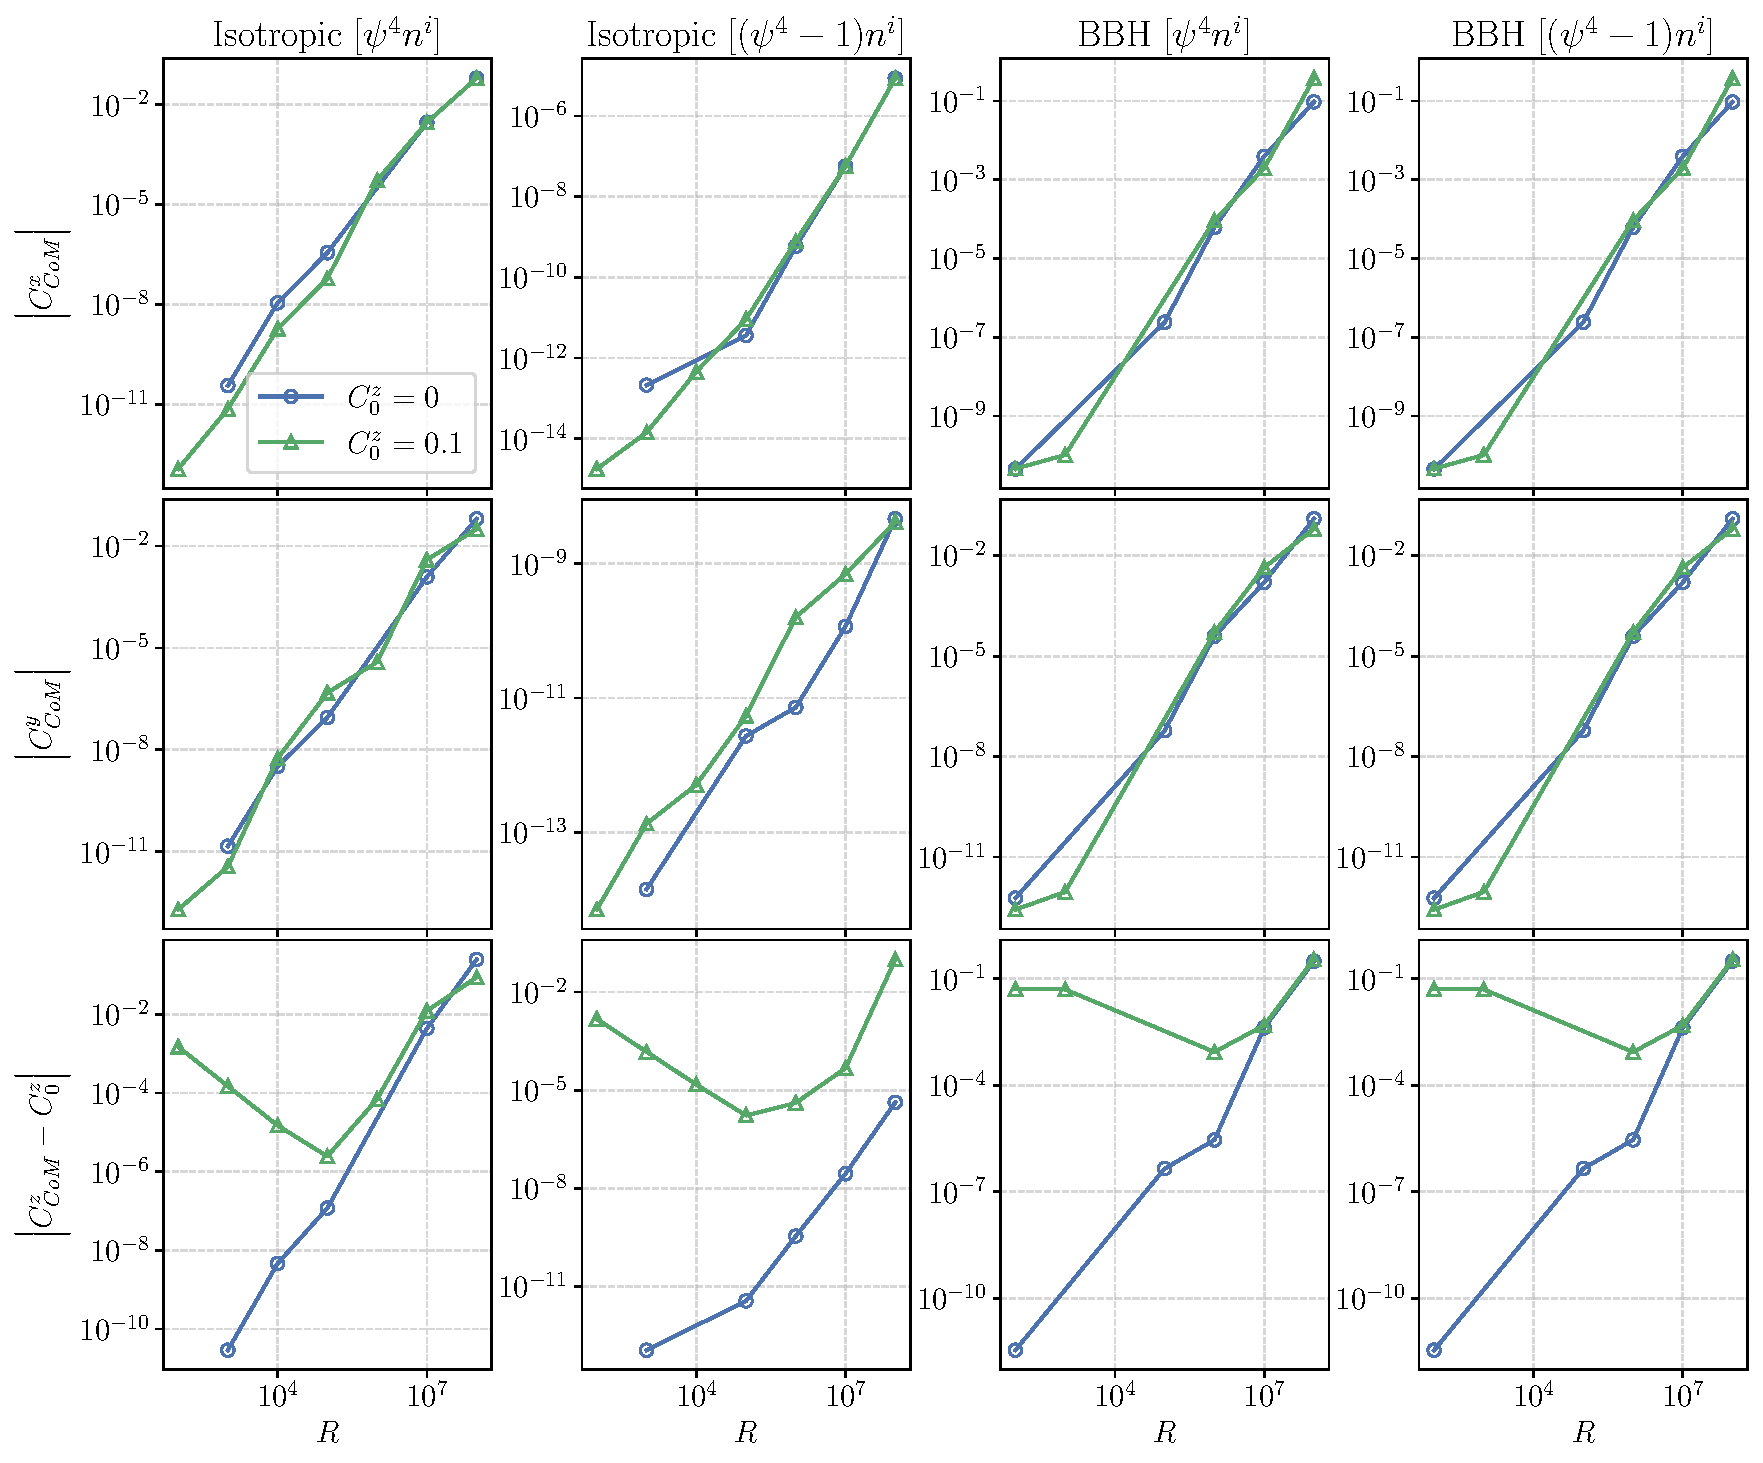
\includegraphics[width=0.85\textwidth]{../../plots/final_report/distance_convergence_CoM_round_off.pdf}
        \caption{Comparison between different versions of the center-of-mass surface integrals. $[\psi^4 n^i]$ refers to \eq{\eqref{eq:CoM-surf}}, while $[(\psi^4-1) n^i]$ refers to \eq{\eqref{eq:CoM-surf-1}}.}
        \label{fig:distance_convergence_CoM_round_off}
      \end{figure}

      We can modify \eq{\eqref{eq:CoM-surf}} in an attempt to address this issue with round-off errors. One way to do this is to transform the integrand $\psi^4 n^i$ to $(\psi^4 - 1) n^i$. Analytically, this should not change the result because
      \begin{align}
        C_\text{CoM}^i
        &= \frac{3}{8 \pi M_\text{ADM}} \oint_{S_\infty} (\psi^4-1) n^i \, dA \label{eq:CoM-surf-1} \\
        &= \frac{3}{8 \pi M_\text{ADM}} \left( \oint_{S_\infty} \psi^4 n^i \, dA - \oint_{S_\infty} n^i \, dA \right) \\
        &= \frac{3}{8 \pi M_\text{ADM}} \oint_{S_\infty} \psi^4 n^i \, dA.
      \end{align}
      Numerically, this makes the terms being cancelled in the calculation smaller. Figure \ref{fig:distance_convergence_CoM_round_off} compares the residuals for each integrand. From this, it is clear that \eq{\eqref{eq:CoM-surf-1}} significantly reduces the round-off errors. Therefore, we use this version for the remaining results of the center-of-mass surface integral.

      \begin{figure}
        \centering
        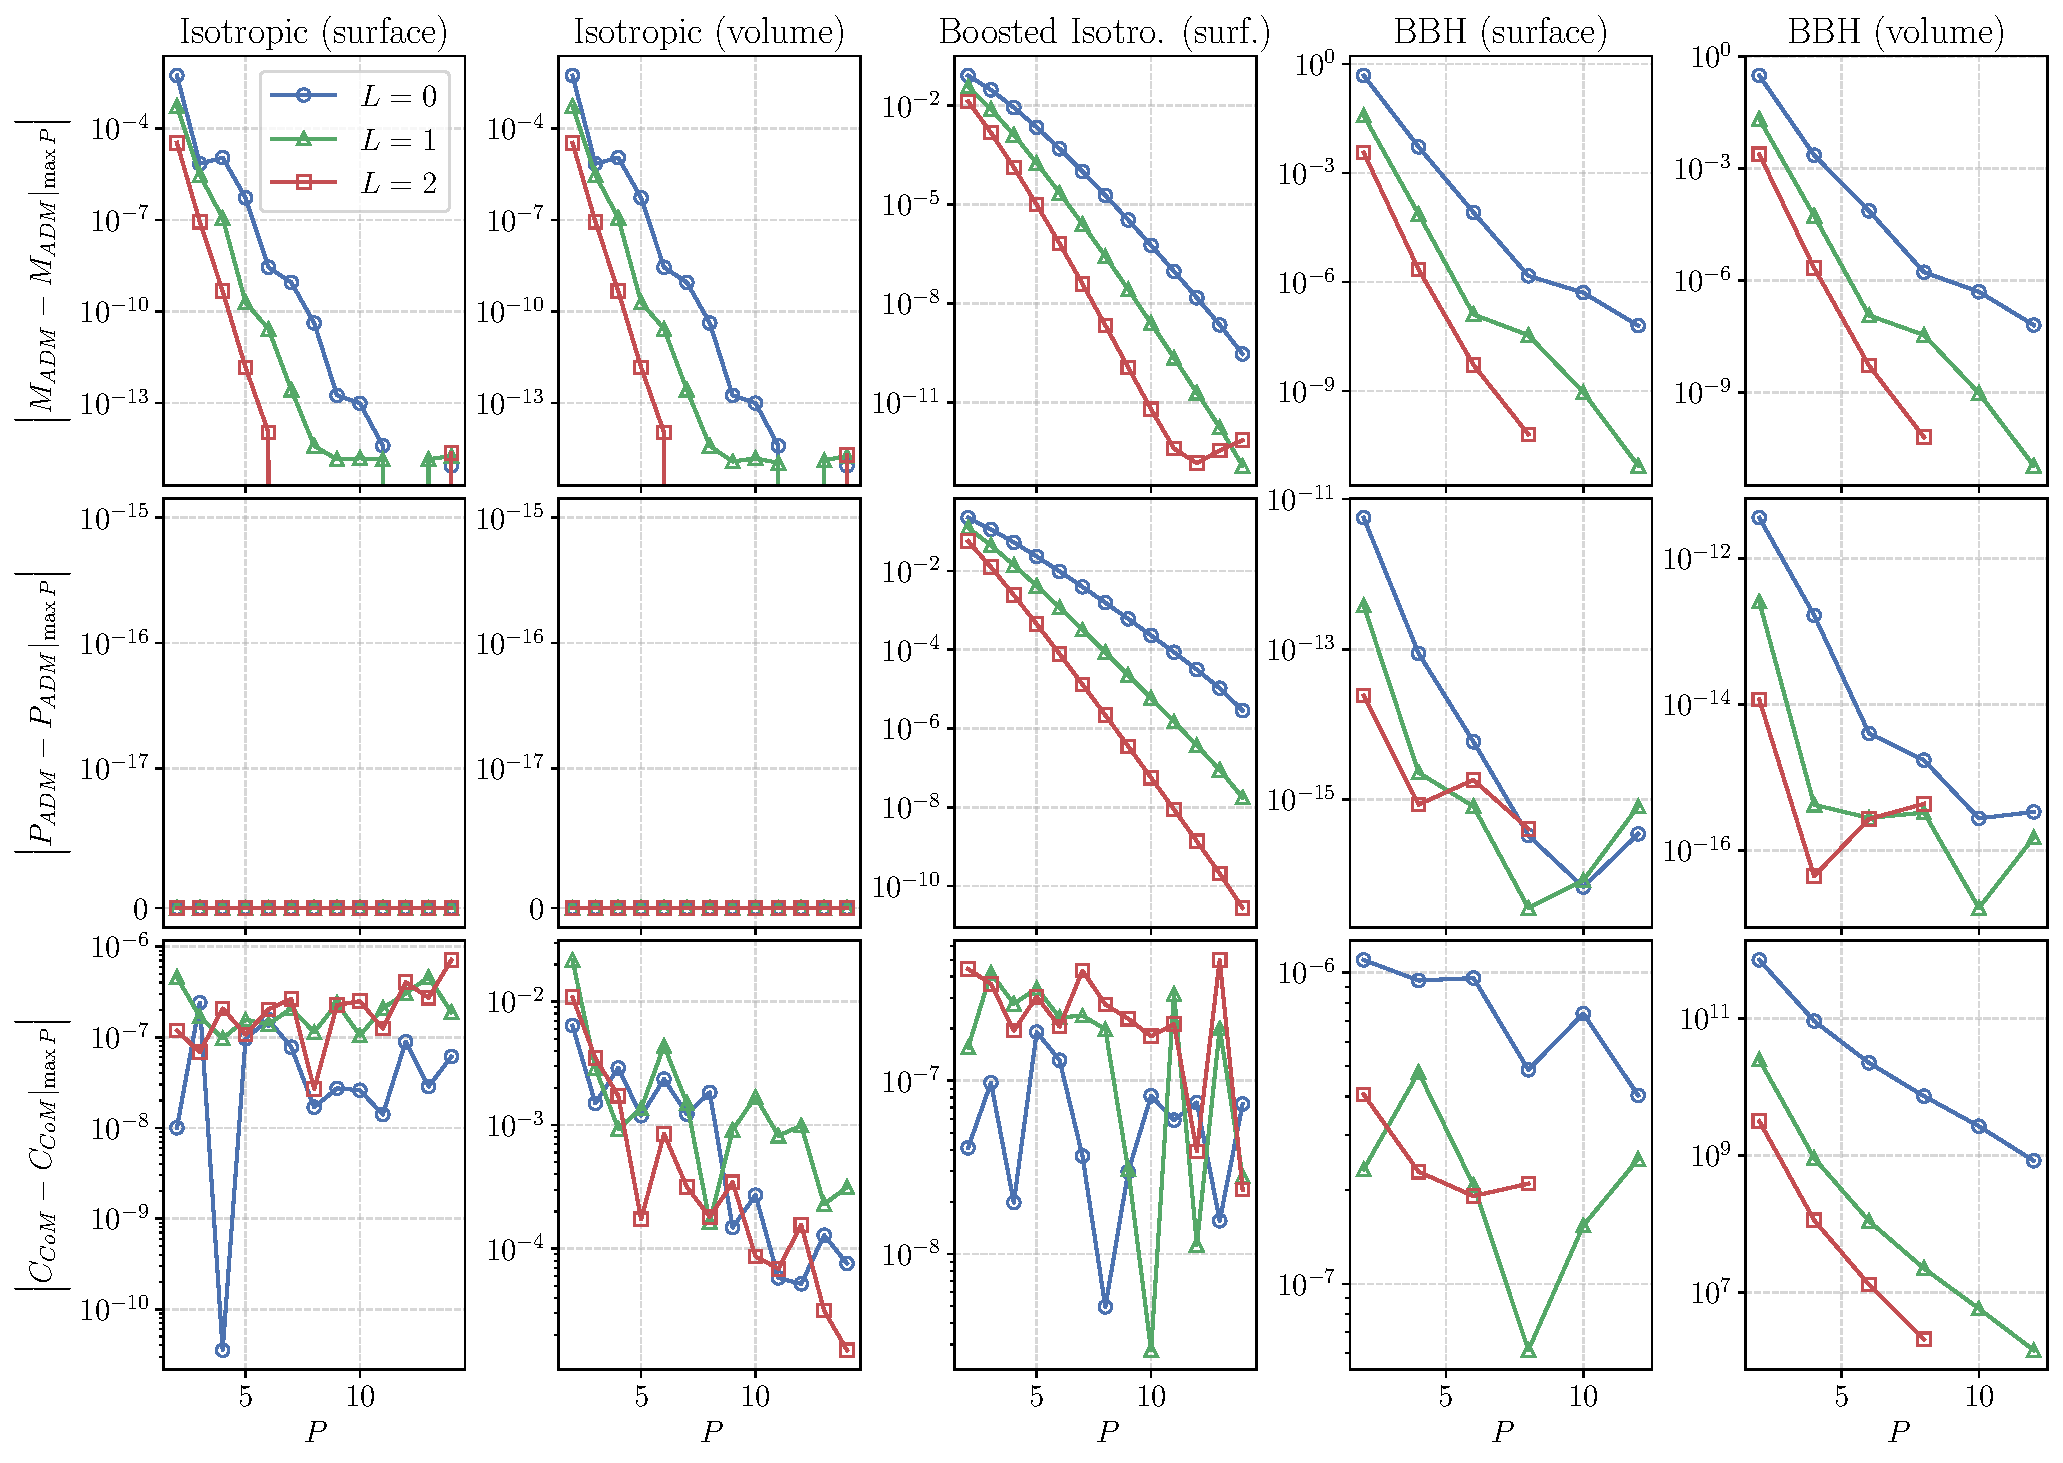
\includegraphics[width=\textwidth]{../../plots/final_report/resolution_convergence.pdf}
        \caption{Convergence with resolution for $M_\text{ADM}$, $P_\text{ADM}$, and $C_\text{CoM}$. Each subplot shows the difference at each polynomial order $P$ relative to the highest $P$ result for multiple refinement levels $L$.}
        \label{fig:resolution_convergence}
      \end{figure}

      Apart from knowing that we approach the expected values for increasing $R$, we must confirm that the results get more accurate with resolution. Figure \ref{fig:resolution_convergence} shows that the residuals in general converge exponentially with polynomial order $P$ and converge faster with higher refinement level $L$, as expected for the Discontinuous Galerkin scheme used in {\tt SpECTRE} \cite{DGMethods}. The center-of-mass convergence plots do not follow this trend, which could be related to the round-off errors, but they still converge as we increase resolution. It is also important to note that the BBH center-of-mass ``volume'' integral has large residuals, which is expected given the $C_\text{CoM}^x$ divergence in Figure \ref{fig:distance_convergence_CoM}.

      The motivation to apply Gauss' divergence theorem in the calculation of the asymptotic quantities was to achieve higher accuracy. Instead of relying on the coarse area elements at the outer boundary (i.e., \eqs{\eqref{eq:Madm-surf}, \eqref{eq:CoM-surf}}, \eqref{eq:Padm-surf}), we can use the more-precise area elements at the inner boundaries along with the volume elements of the entire domain (i.e., \eqs{\eqref{eq:Madm-mixed}--\eqref{eq:Padm-mixed}}). However, Figure \ref{fig:resolution_convergence} shows that we did not get much benefit out of this transformation. The ADM masses appear to be almost identical between the surface and volume results. The ADM linear momenta have slightly lower residuals for the BBH volume results compared to the surface ones, but nothing too significant. The centers of mass as volume integrals have higher round-off errors than their surface counterparts, and we see occasional blow-ups in the volume version.

      Therefore, the volume integrals do not seem favorable for our purposes at the current stage. In {\tt SpEC}, this transformation was used in the computation of the ADM linear momentum $\vec P_\text{ADM}$ and the ADM angular momentum $\vec J_\text{ADM}$ \cite{Serguei}. There, accuracy was improved by one order of magnitude for $\vec P_\text{ADM}$ and by several orders of magnitude for $\vec J_\text{ADM}$ \cite{Serguei}. That said, it is important to note that {\tt SpEC}'s BBH outer boundary is $R \sim 10^{10}$ \cite{Serguei}, while {\tt SpECTRE}'s is $R \sim 10^5$ due to its better boundary conditions \cite{Vu_2024}. The smaller outer boundary might explain why we don't see a significant improvement when using the $\vec P_\text{ADM}$ volume integrals. We plan to compute $\vec J_\text{ADM}$ in the future, so it is worth re-evaluating this at that time.

    \subsection{Control of BBH parameters}

      \begin{table}
        \centering
        \def\arraystretch{1.5}
		    \setlength{\tabcolsep}{0.5cm}
        \begin{tabular}{lccc}
          \hline
          \hline
          Name & $q$ & $\vec \chi^*_A$ & $\vec \chi^*_B$ \\
          \hline
          {\tt q1} & 1 & (0,0,0) & (0,0,0) \\
          {\tt q3} & 3 & (0,0,0) & (0,0,0) \\
          {\tt q3-spin} & 3 & (0,0,0.9) & (0,0,0) \\
          \hline
          \hline
        \end{tabular}
        \caption{Target parameters of the BBH runs. The masses $M^*_{A,B}$ are determined by the mass ratio $q = M^*_A / M^*_B$ and $M^*_A + M^*_B = 1$.}
        \label{tab:bbh-runs}
      \end{table}

      To test our control loop, we ran three BBH cases. Table \ref{tab:bbh-runs} shows the target parameters for each of these runs. Figure \ref{fig:control_iterations} shows how many control iterations were needed for each run as well as how the control residual ${\bf F}({\bf u})$ behaved. We finish the control loop when the largest component of ${\bf F}({\bf u})$ reaches the residual tolerance of $10^{-6}$. From these results, it is clear that our control scheme finished in very few iterations and was able to handle scenarios from a simple equal-mass non-spinning run to a non-trivial mass ratio with high spin.

      \begin{figure}
        \centering
        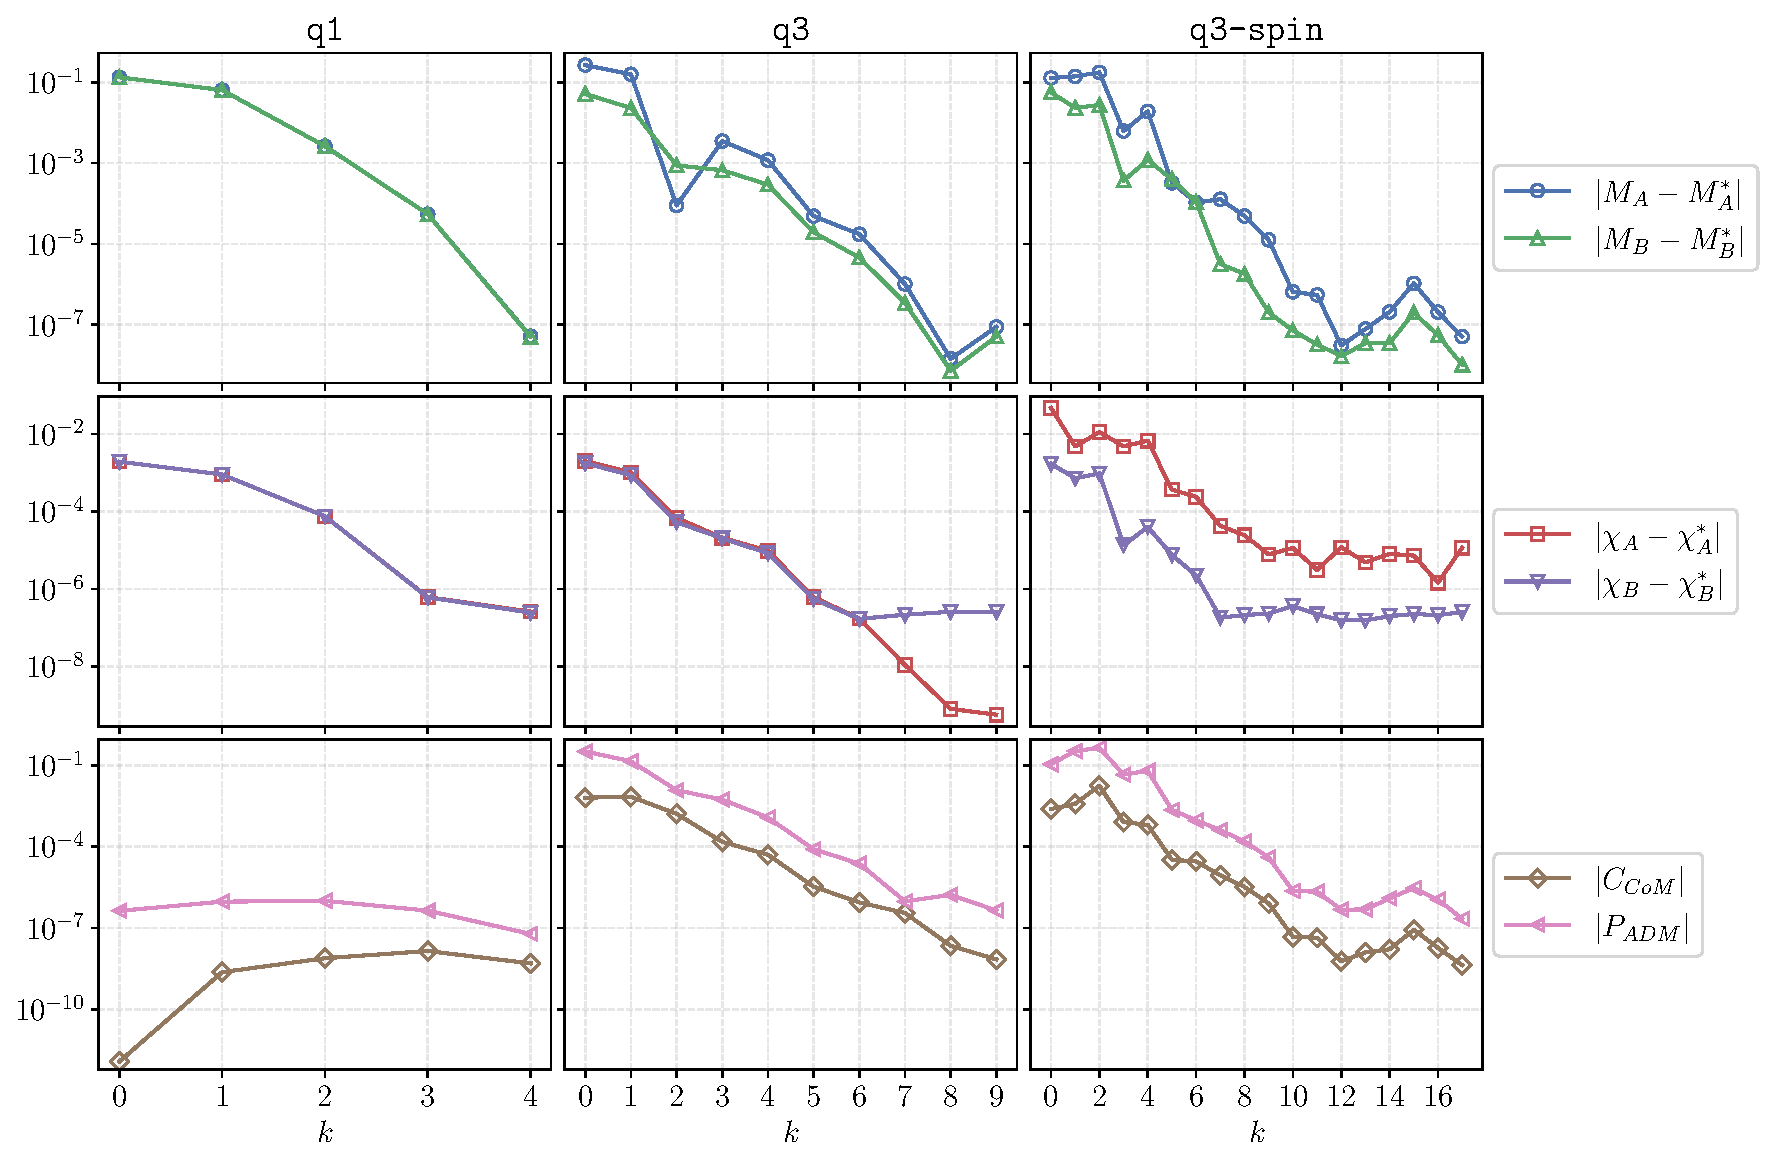
\includegraphics[width=0.85\textwidth]{../../plots/final_report/control_iterations.pdf}
        \caption{Control results for the BBH runs shown in Table \ref{tab:bbh-runs}. The control residuals ${\bf F}({\bf u})$ are shown for each control iteration $k$. Here, $\vec C_\text{CoM}$ and $\vec P_\text{ADM}$ were computed using \eq{\eqref{eq:CoM-surf-1}} and \eq{\eqref{eq:Padm-surf}}.}
        \label{fig:control_iterations}
      \end{figure}

      We attempted to run the BBH cases shown in Table 1 of \cite{Serguei}, but we did not succeed. For the {\tt Spin0.9999} and {\tt q10} runs, {\tt SpECTRE}'s horizon finder failed after the first XCTS solve. There was a recent update to the {\tt SpECTRE} BBH domain, which might have fixed such problems. For the {\tt q3} and {\tt q10} runs, the free data updated by \eq{\eqref{eq:u-iteration}} contained invalid values like negative masses and $\chi > 1$. This could be fixed by adding constraints to the iterative loop, making sure that the free data stays within an acceptable range.

  \section{Conclusion}

    {\tt SpECTRE} is now capable of controlling physical parameters in BBH initial data. Our control scheme not only enforces specific masses and spins for the desired simulation, but also avoids drifts in the orbital trajectories by minimizing the center of mass and the total linear momentum. For this, we had to compute asymptotic quantities defined as infinite integrals, which can be cast as surface integrals or volume integrals. In general, we have found that the volume integrals lead to either similar or worse residuals when compared to the surface integrals. The integral results for the total energy and linear momentum converge nicely. Although the integral results for the center of mass have some issues that must be investigated, the surface integral achieves acceptable residuals for the current applications.

  \section{Future work}

    There are many possible improvements to the work described in this report. For instance, we plan to find ways to get around the round-off errors observed in the center-of-mass integrals. This could include changes to the integral itself, like in \eq\eqref{eq:CoM-surf-1}, or alternative integration methods, such as the spectral integration done in {\tt SpEC} \cite{Serguei}. We should also make the control scheme more rigorous with constraints for the free data and more efficient with optimizations like line search, allowing {\tt SpECTRE} to reach more of the parameter space.

    There is also a lot of interest in follow-up work. For example, it is important to understand whether we have made significant improvements in our control scheme relative to the one used by {\tt SpEC}, either in terms of performance or parameter space. To this purpose, we need to do a careful comparison between the two codes. Additionally, by implementing the computation of total angular momentum $\vec J_\text{ADM}$, we would be able to control $M_\text{ADM}$ and $\vec J_\text{ADM}$ to generate initial data for BBH hyperbolic encounters.

    Improving performance is also of great interest. Like in {\tt SpEC}, it would be desirable to start the control scheme at a lower resolution and increase it to the desired one only when needed. Along with that, we could use the solution from the previous control iteration as an initial guess to the following XCTS solve. We could also reduce the number of control iterations needed by starting with better free data than \eq{\eqref{eq:u0}}, provided by a machine learning algorithm that models ${\bf F}({\bf u})$.

    Finally, {\tt SpECTRE} BBH runs initially have junk radiation that affects the effective simulation parameters $M_{A,B}$, $\vec \chi_{A,B}$, $\vec C_\text{CoM}$, and $\vec P_\text{ADM}$ on the order of $10^{-3}$ \cite{Serguei}. There have been attempts to minimize these effects by starting with a configuration that will result in the target parameters after junk radiation leaves domain \cite{Higginbotham:2019}. Implementing such an after-junk control scheme in {\tt SpECTRE} would be of high value, which could look like a statistical fitting model motivated by single black holes (like in \cite{Higginbotham:2019}) or a machine learning algorithm that models the effects of junk radiation.

  \section*{Acknowledgements}

    I am extremely thankful to my mentors for the constant support during and beyond the extent of the Caltech SURF program. I would also like to thank my mentor and advisor at Oberlin College, Robert Owen, for many helpful discussions and for coming up with the idea used in \eq{\eqref{eq:CoM-surf-1}}. I am also grateful to all the faculty, postdocs and graduate students with whom I connected over the duration of the program. Computations were
    performed with the Resnick High-Performance Computing Center cluster at Caltech.

  \section*{References}

	  \printbibliography[heading=none]
  
\end{document}
